\apendice{Documentación técnica de programación}

\section{Introducción}

\section{Estructura de directorios}

\section{Manual del programador}

\section{Compilación, instalación y ejecución del proyecto}

\section{Compilación, instalación y ejecución de herramientas auxiliares}

\subsection{KEEL}

KEEL es una herramienta que permite experimentar con modelos de \textit{machine learning}. Ha sido creada por distintas universidades españolas y financiada por el Ministerio de Educación y Ciencia~\cite{KEEL}.

Para poder ejecutarla, en primer lugar, se han de descargar los ficheros fuente del repositorio de GitHub~\cite{keelRepo}. Una vez se han descargado, se compilan aprovechando el fichero \texttt{build.xmlz} contenido y la herramienta \texttt{ant}. Mediante el comando \texttt{ant cleanAll} se eliminan barios previos (para evitar conflictos), y mediante el comando \texttt{ant} se compila el código fuente.

Posteriormente se ejecuta la aplicación mediante el comando \texttt{java -jar ./dist/GraphInterKeel.jar} y se utiliza mediante su interfaz gráfica.

\begin{figure}[h]
	\caption[\textit{Co-forest}: Configuración de un experimento en KEEL]{Configuración de un experimento que utiliza el algoritmo \textit{co-forest} mediante la GUI de KEEL.}
	\centering
	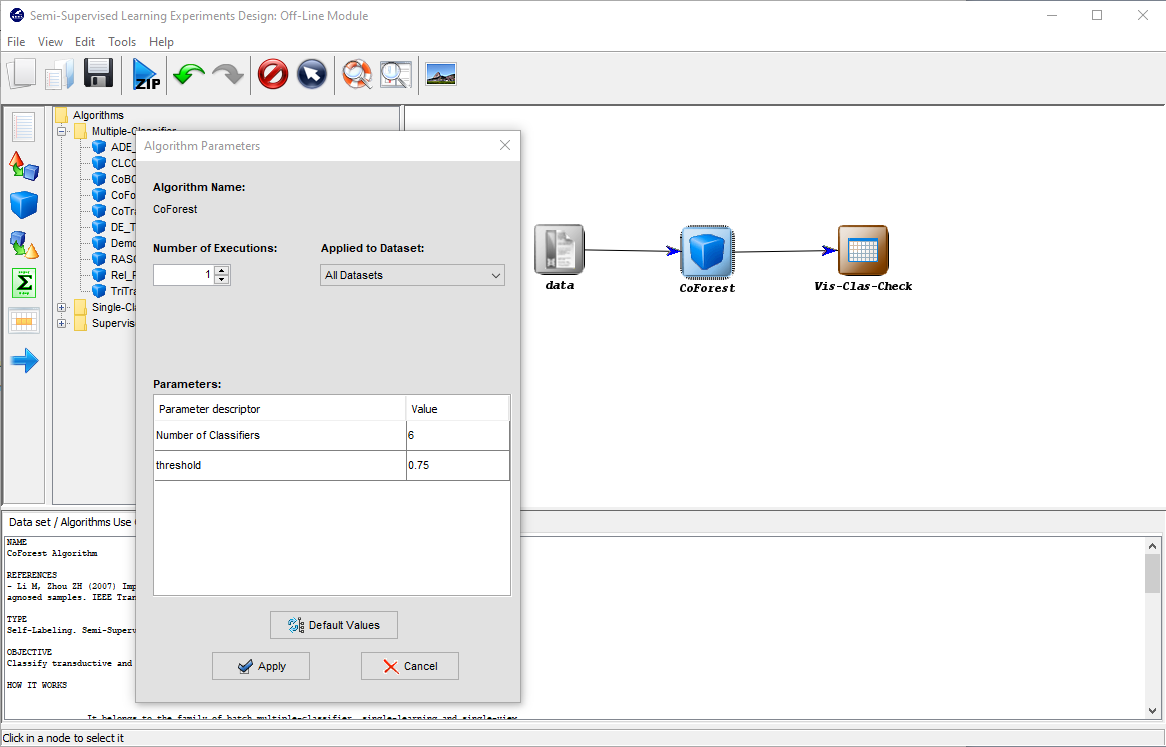
\includegraphics[width=\textwidth]{../img/anexos/manual/keel_gui.png}
\end{figure}


\section{Pruebas del sistema}
\label{s:pruebas}

\subsection{Pruebas unitarias}
\label{s:pruebas-unitarias}
Travis...

\subsection{Pruebas de aceptación}
\label{s:pruebas-aceptación}

\begin{table}[p]
	\centering
	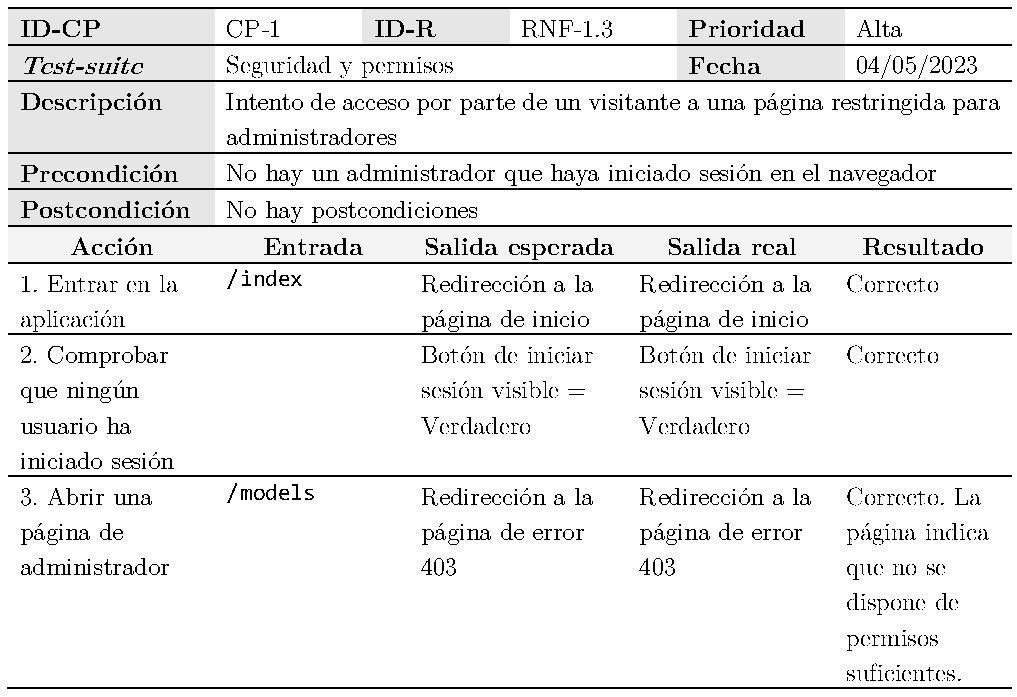
\includegraphics[width=\textwidth]{../img/anexos/cp/CP-1}
	\caption{CP-1 Acceso a página restringida.}
	\label{cp:acc-restringido}
\end{table}

\begin{table}[p]
	\centering
	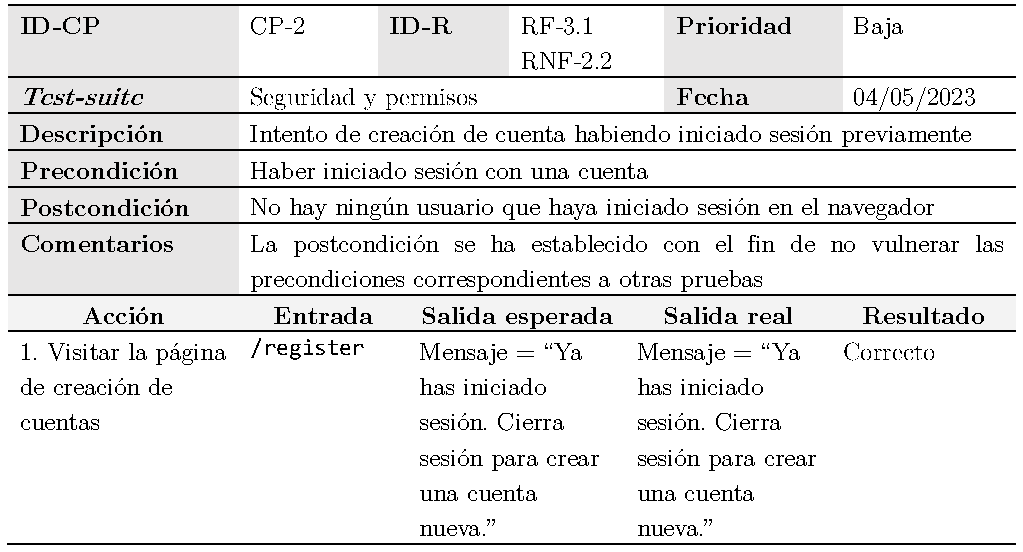
\includegraphics[width=\textwidth]{../img/anexos/cp/CP-2}
	\caption{CP-2 Intento de registro con cuenta accedida.}
	\label{cp:registro}
\end{table}

\begin{table}[p]
	\centering
	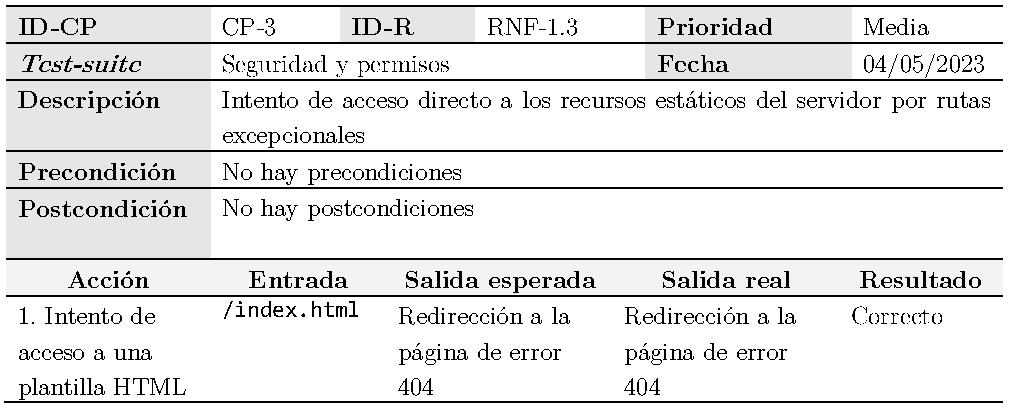
\includegraphics[width=\textwidth]{../img/anexos/cp/CP-3}
	\caption{CP-3 Acceso a recursos estáticos.}
	\label{cp:acc-html}
\end{table}

\begin{table}[p]
	\centering
	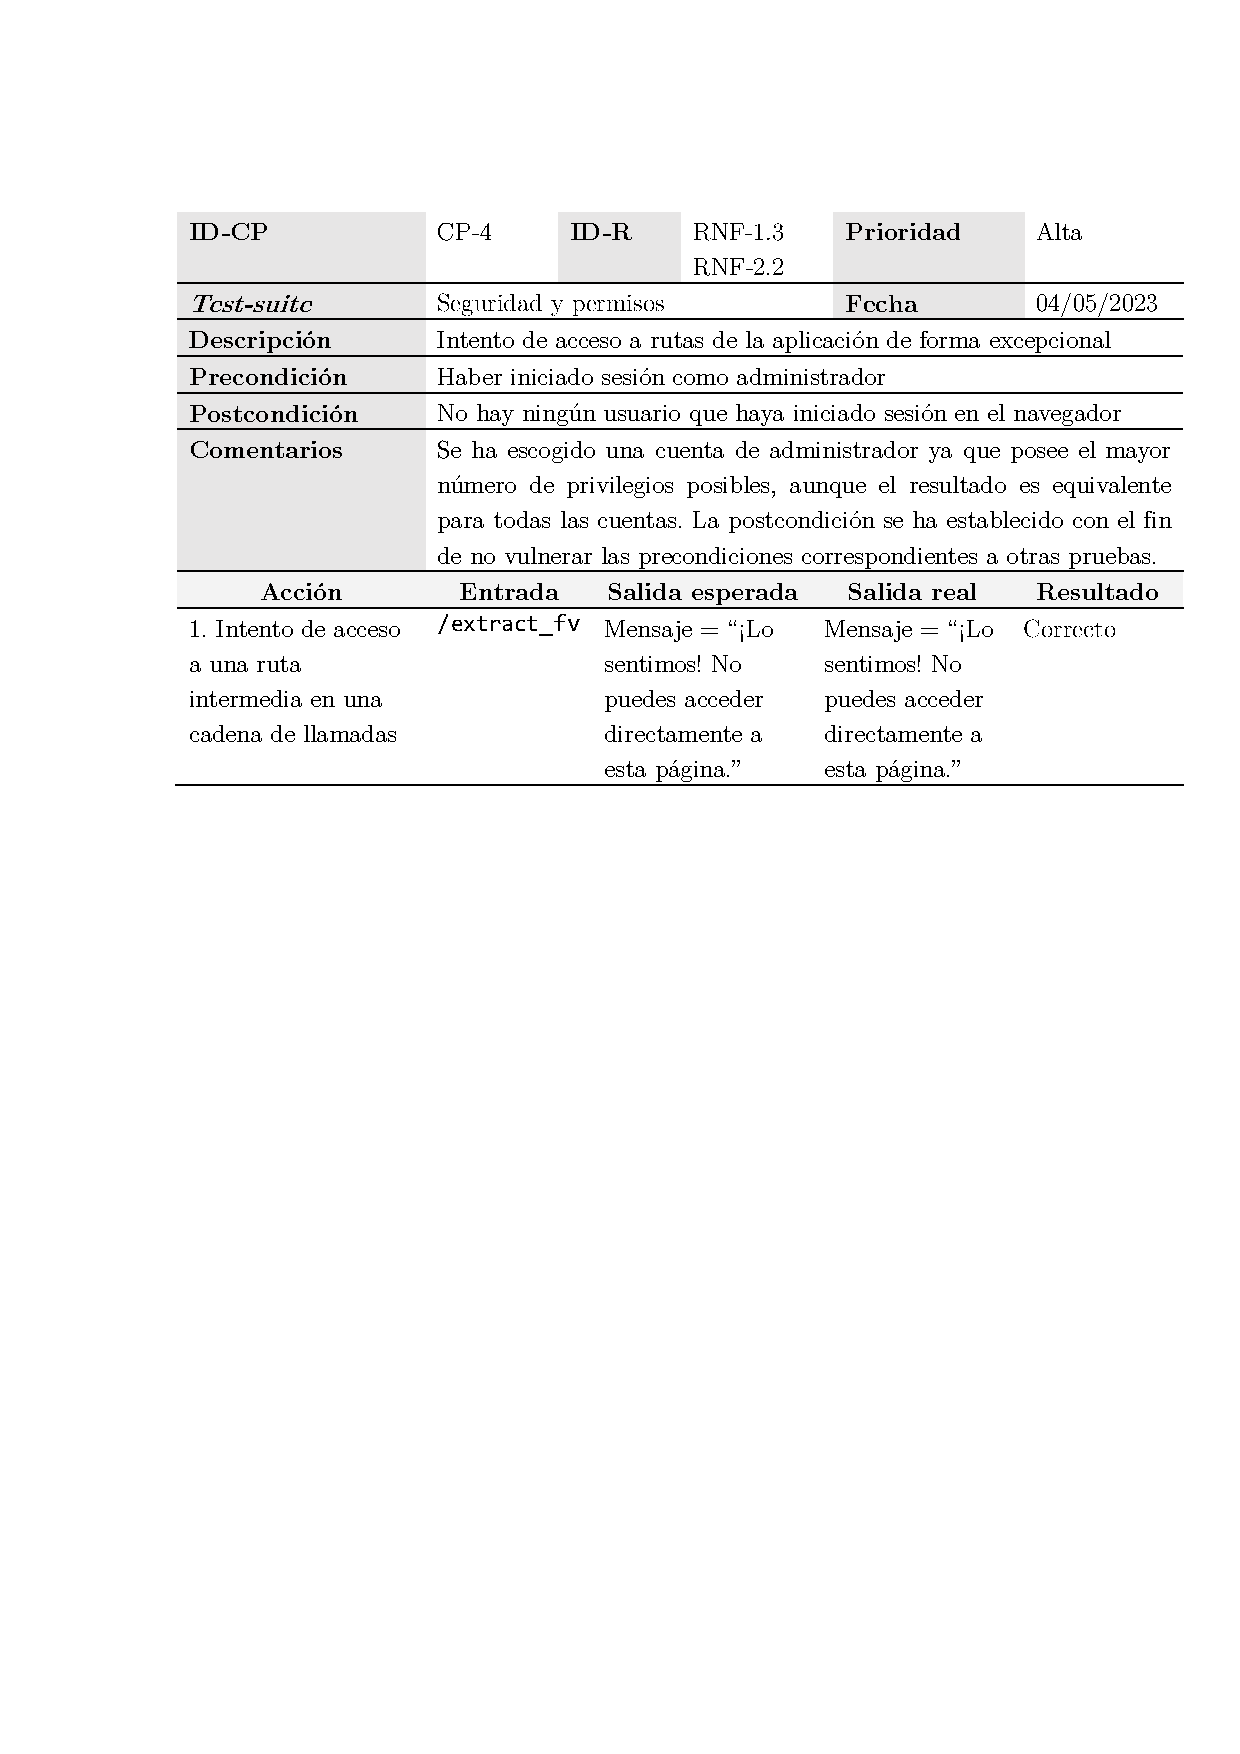
\includegraphics[width=\textwidth]{../img/anexos/cp/CP-4}
	\caption{CP-4 Acceso a rutas excepcionales.}
	\label{cp:wrong-stream}
\end{table}

\begin{table}[p]
	\centering
	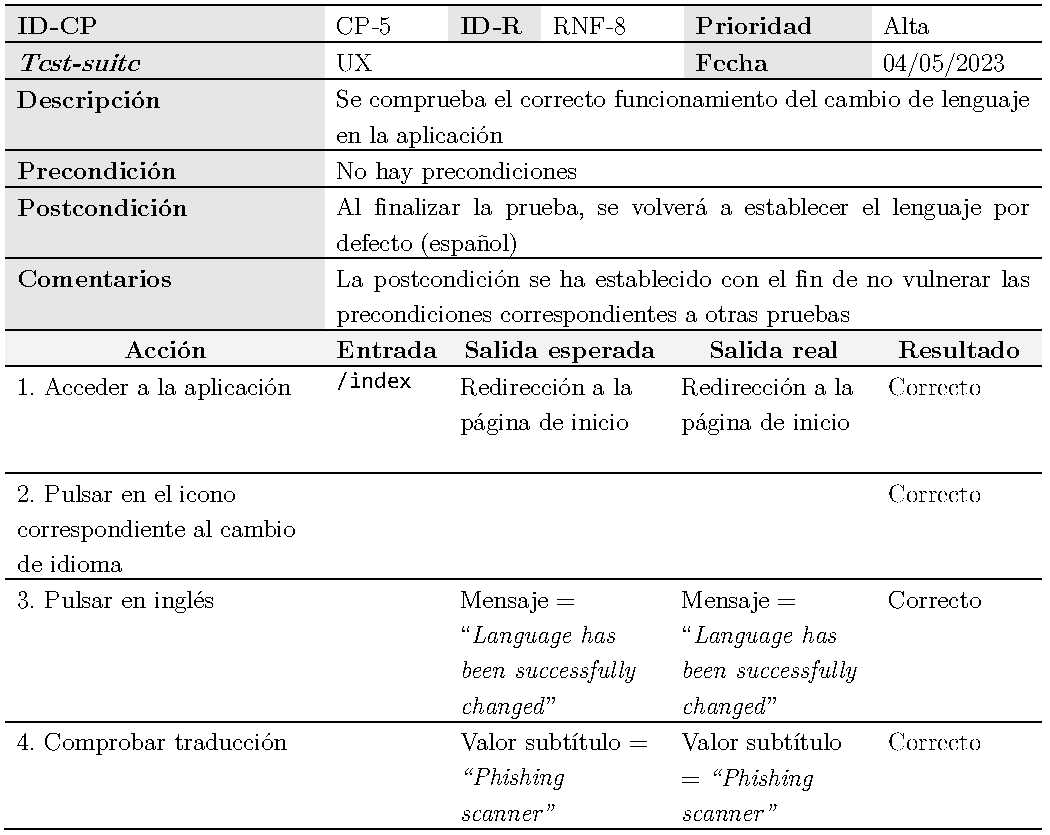
\includegraphics[width=\textwidth]{../img/anexos/cp/CP-5}
	\caption{CP-5 Cambio de lenguaje.}
	\label{cp:language}
\end{table}

\begin{table}[p]
	\centering
	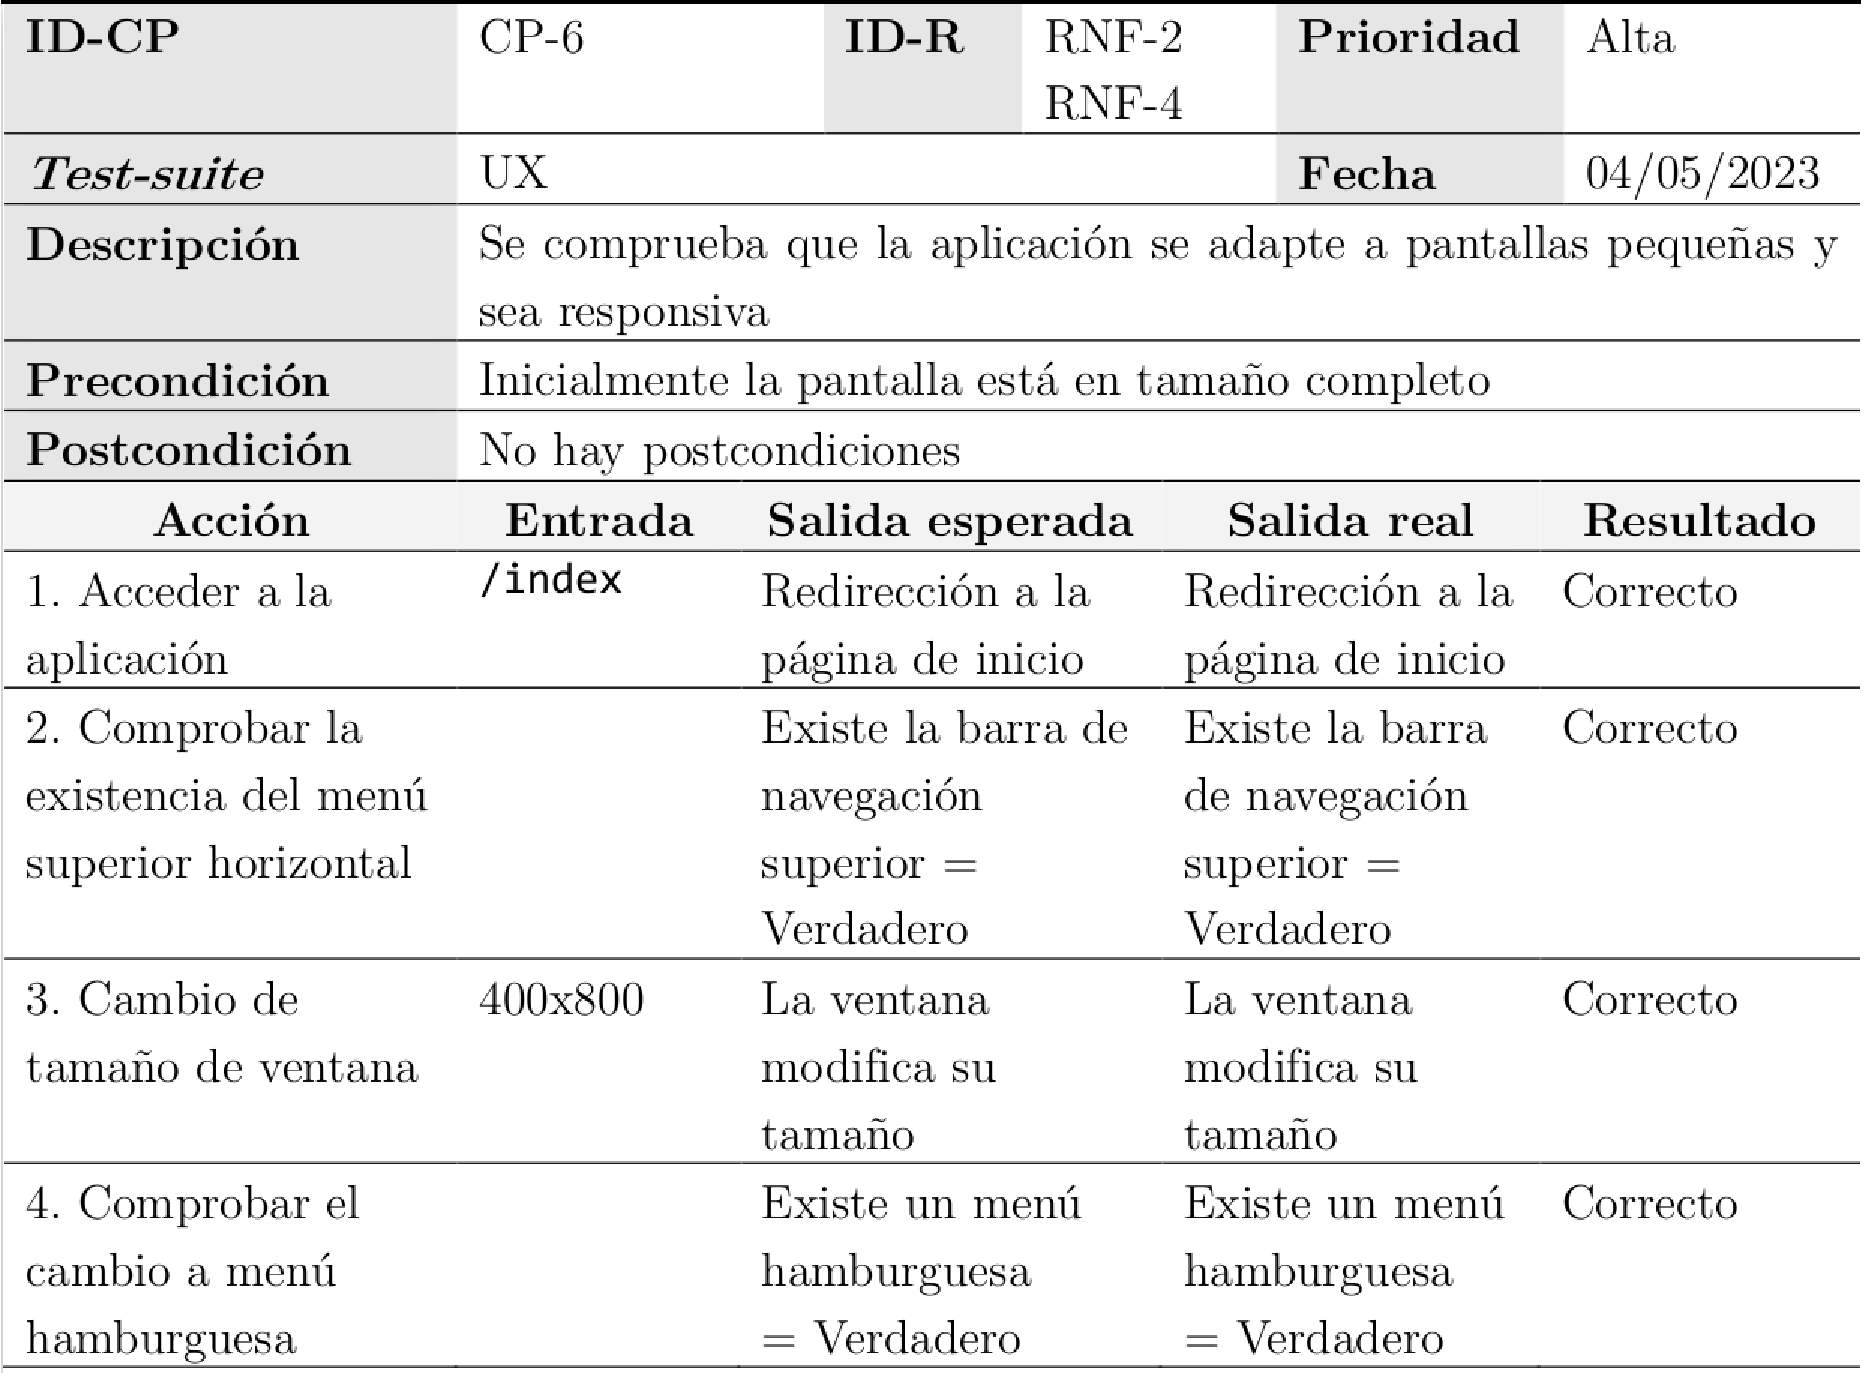
\includegraphics[width=\textwidth]{../img/anexos/cp/CP-6}
	\caption{CP-6 Pantallas responsivas.}
	\label{cp:hamburguer-menu}
\end{table}

\begin{table}[p]
	\centering
	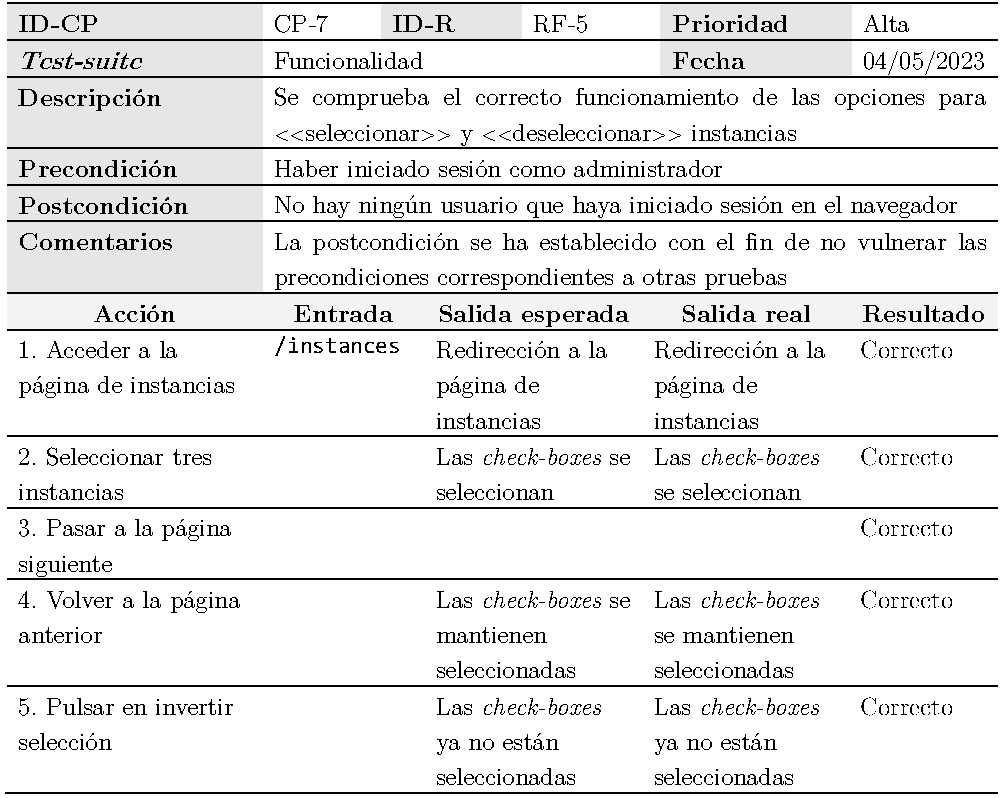
\includegraphics[width=\textwidth]{../img/anexos/cp/CP-7}
	\caption{CP-7 Funcionamiento de las \textit{check-boxes}.}
	\label{cp:checkboxes}
\end{table}

\begin{table}[p]
	\centering
	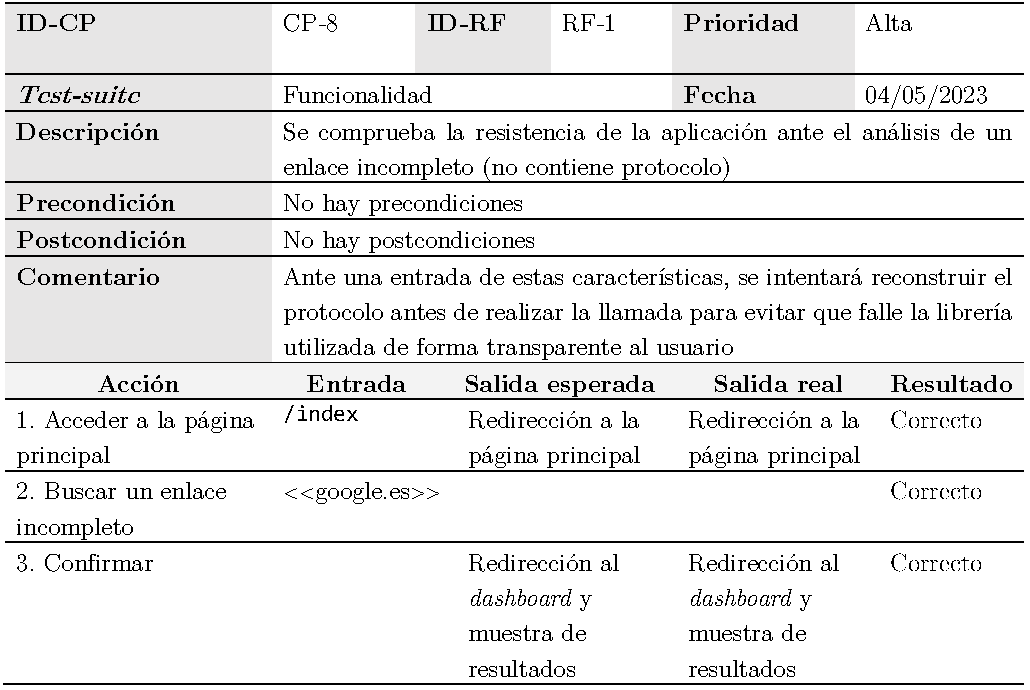
\includegraphics[width=\textwidth]{../img/anexos/cp/CP-8}
	\caption{CP-8 Análisis enlace incompleto.}
	\label{cp:url-incompleta}
\end{table}

\begin{table}[p]
	\centering
	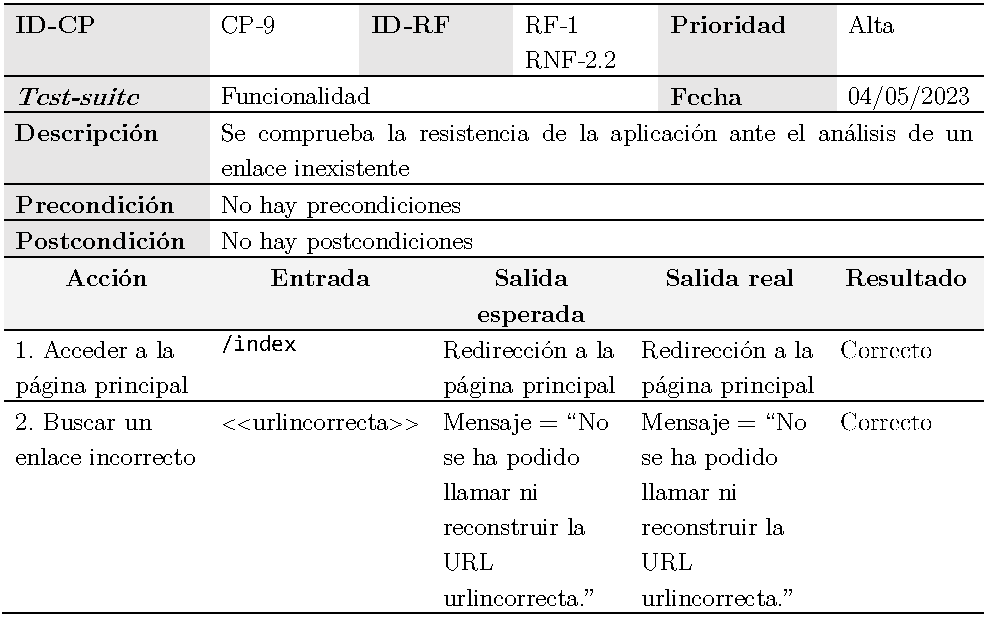
\includegraphics[width=\textwidth]{../img/anexos/cp/CP-9}
	\caption{CP-9 Análisis enlace erróneo.}
	\label{cp:wrong-url}
\end{table}

\begin{table}[p]
	\centering
	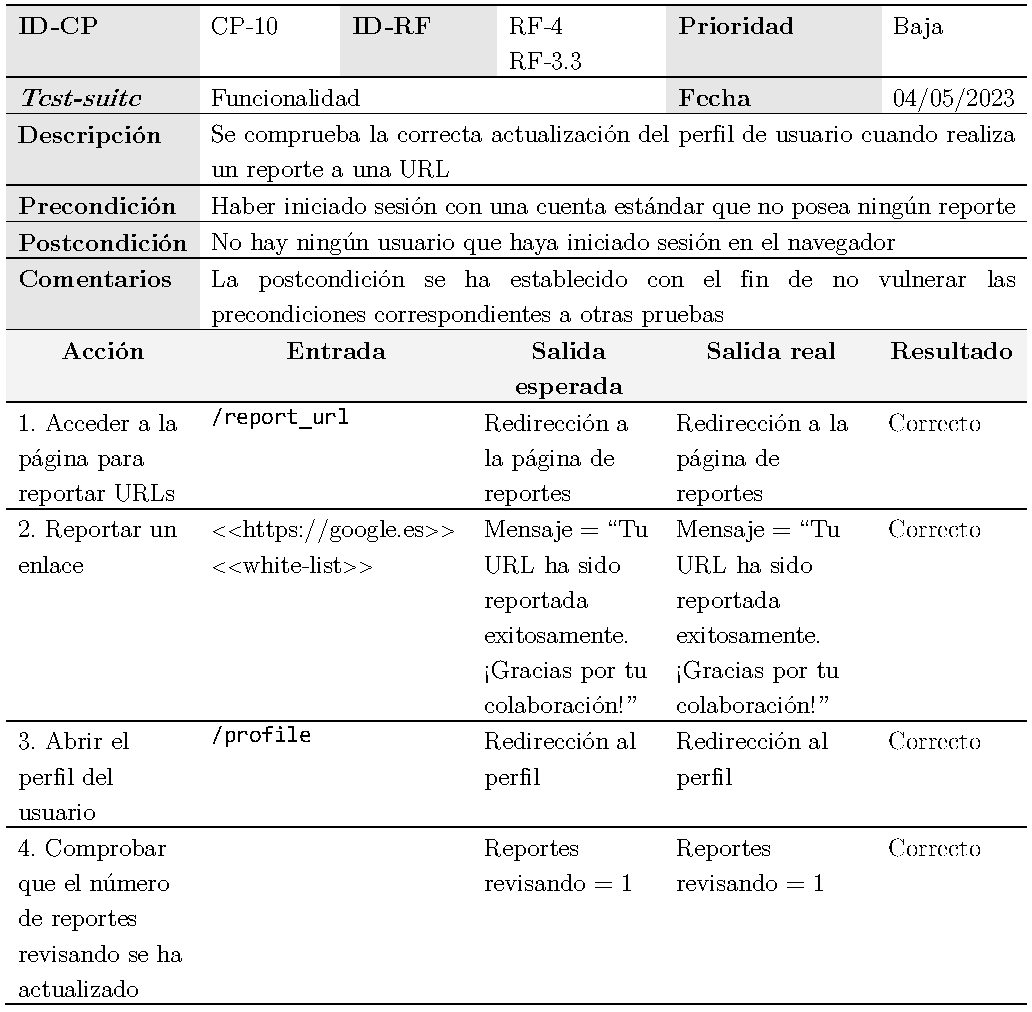
\includegraphics[width=\textwidth]{../img/anexos/cp/CP-10}
	\caption{CP-10 Actualización del perfil con las denuncias de URLs.}
	\label{cp:report-url}
\end{table}

\begin{table}[p]
	\centering
	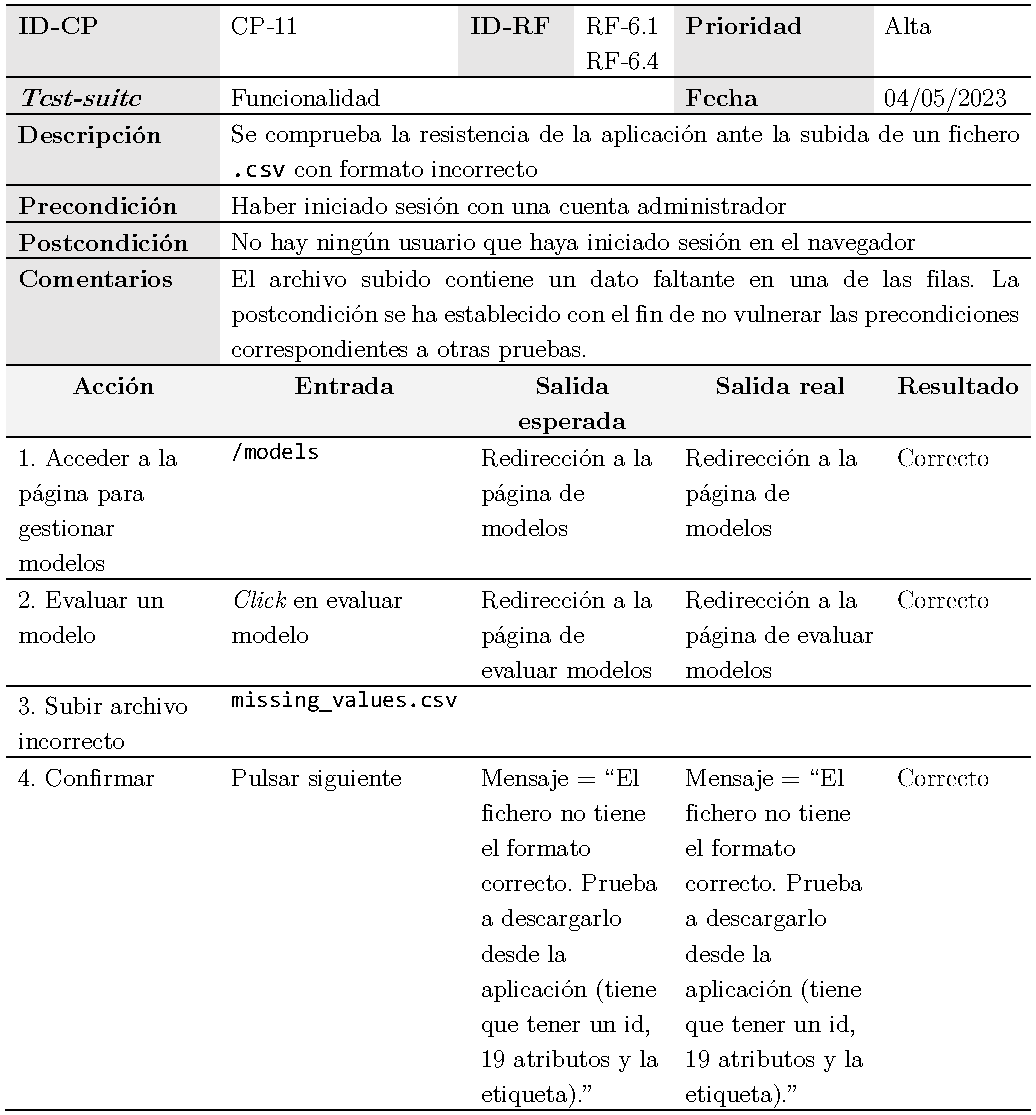
\includegraphics[width=\textwidth]{../img/anexos/cp/CP-11}
	\caption{CP-11 \texttt{csv} con formato incorrecto.}
	\label{cp:wrong-csv}
\end{table}

\begin{table}[p]
	\centering
	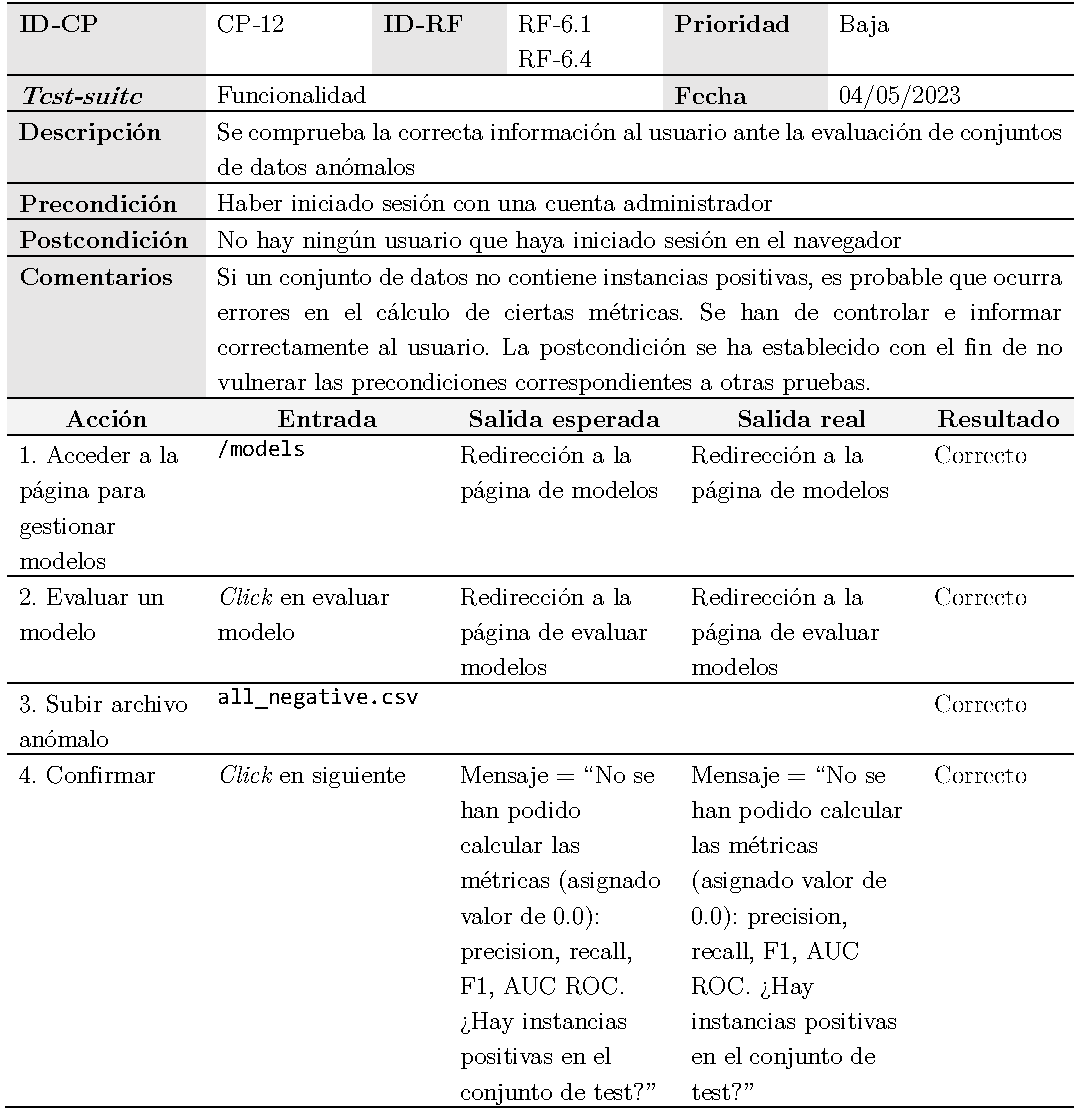
\includegraphics[width=\textwidth]{../img/anexos/cp/CP-12}
	\caption{CP-12 \texttt{csv} con conjunto de \textit{test} anómalo.}
	\label{cp:strange-csv}
\end{table}